\documentclass[9pt,twocolumn,twoside,lineno]{pnas-new}

%% Some pieces required from the pandoc template
\providecommand{\tightlist}{%
  \setlength{\itemsep}{0pt}\setlength{\parskip}{0pt}}

% Use the lineno option to display guide line numbers if required.
% Note that the use of elements such as single-column equations
% may affect the guide line number alignment.


\usepackage[T1]{fontenc}
\usepackage[utf8]{inputenc}

\usepackage{eso-pic,graphicx,transparent}

\templatetype{pnasresearcharticle}  % Choose template

\title{The Regional Effects of Marine Protected Areas}

\author[a,1]{Daniel Ovando}
\author[b]{Jennifer E. Caselle}
\author[b]{Christopher Costello}
\author[b]{Olivier Deschenes}
\author[b]{Steven D. Gaines}
\author[a]{Ray Hilborn}
\author[b]{Owen Liu}

  \affil[a]{University of Washington, School of Aquatic and Fishery Science}
  \affil[b]{University of California, Santa Barbara}


% Please give the surname of the lead author for the running footer
\leadauthor{Ovando}

% Please add here a significance statement to explain the relevance of your work
\significancestatement{Healthy marine ecosystems are critical to the well-being of the planet.
Marine protected areas, parts of the oceans protected from human
activities such as fishing, are increasingly being used in an effort to
conserve and manage these ecosystems. Our study pairs theory with
empirical methods to examine the regional effects of MPAs on
conservation and fishery outcomes. Using simulations, we show that the
effects of marine protected areas can be highly variable and dependent
on human drivers. Building off of MPA theory, we find no statistically
clear effect of a network of MPAs, which our simulation analysis
suggests is entirely reasonable. Our results lay a foundation for future
research on the design and monitoring of marine protected areas.}


\authorcontributions{D.O., S.G., and R.H. developed structure of simulation model. D.O.,
O.D., C.C., and J.C. developed estimation strategy. J.C. provided
support on collecting and interpreting data. All simulations,
statistics, and sensitivity analyses performed by D.O. and O.L. . All
authors contributed to the manuscript.}

\authordeclaration{R.H's research program receives funding from environmental NGOs,
foundations, fishing industry, governments and international agencies.
All of these can be interpreted as a conflict of interest when
evaluating fisheries policy. C.C., S.G., and O.D's research program
includes funding from environmental NGOs and foundations with an
interest in ocean conservation and food security}


\correspondingauthor{\textsuperscript{} }

% Keywords are not mandatory, but authors are strongly encouraged to provide them. If provided, please include two to five keywords, separated by the pipe symbol, e.g:
 \keywords{  Marine Protected Areas |  Conservation |  Bio-economic modeling |  Program Evaluation |  Channel Islands National Marine Sanctuary  } 

\begin{abstract}
Marine Protected Areas (MPAs) cover between 3-7\% of the world's oceans,
up from less than 1\% in the year 2000. The Convention on Biological
Diversity calls for 10\% of coastal waters to be protected inside MPAs
by 2020, while the International Union for Conservation of Nature calls
for 30\% protection by 2030. It is often clear that MPAs produce
conservation benefits inside their borders, but many MPAs are also
justified on the grounds that they also benefit the broader region
outside their borders. Despite the expanding role of MPAs in marine
resource management, we lack a clear understanding of what the regional
effects of MPAs might be, and how we might detect them in scientific
studies. We used a bio-economic simulation model to demonstrate how the
regional effects of MPAs are affected by a suite of economic and
environmental drivers and show how commonly used methods to measure
inside-MPA effects are likely to fail to capture the regional impacts of
protection. We present an empirical strategy for estimating regional MPA
effects on biomass density using 16 years of data from inside and
outside of MPAs within the Channel Islands, California, USA. We find no
statistically clear effect of MPAs on aggregate mean biomass densities
of targeted finfish throughout the study region. To make meaningful
progress on MPA design and evaluation, the next generation of MPA
science must address the challenge of understanding and estimating the
regional effects of MPAs across the diversity of species in the
ecosystem.
\end{abstract}

\dates{This manuscript was compiled on \today}
\doi{\url{www.pnas.org/cgi/doi/10.1073/pnas.XXXXXXXXXX}}

\begin{document}

% Optional adjustment to line up main text (after abstract) of first page with line numbers, when using both lineno and twocolumn options.
% You should only change this length when you've finalised the article contents.
\verticaladjustment{-2pt}

\maketitle
\thispagestyle{firststyle}
\ifthenelse{\boolean{shortarticle}}{\ifthenelse{\boolean{singlecolumn}}{\abscontentformatted}{\abscontent}}{}

% If your first paragraph (i.e. with the \dropcap) contains a list environment (quote, quotation, theorem, definition, enumerate, itemize...), the line after the list may have some extra indentation. If this is the case, add \parshape=0 to the end of the list environment.

\acknow{This study would not be possible without the work provided by PISCO
divers over the years. DO thanks Cody Szuwalski, Julia Lawson, and André
Punt for helpful comments and technical support.}

\correspondingauthor{\textsuperscript{1}To whom correspondence should be addressed. E-mail: danovan@uw.edu}

No-take Marine Protected Areas (MPAs), spatial regions of the ocean in
which fishing is prohibited, have a long history in the management of
marine resources. Traditional cultures in Oceania utilized - often
temporary - MPAs as ``fish banks'' for times of need (1). Modern MPAs
were first established primarily as marine analogs to the terrestrial
protection of iconic landscapes like Yellowstone or Kruger National
Parks (2, 3). Over time our goals and expectations for MPAs have
evolved; while all MPAs are expected to deliver conservation benefits
within their borders, many modern MPAs are also established to bolster
fish populations throughout the region in which they are located (what
we term ``regional-scale effects'') (4).

Indeed, many recent agreements to expand MPAs (most proximately, the
Convention on Biological Diversity's Strategic Plan for Biodiversity,
which calls for 10\% of coastal waters to be protected inside MPAs by
2020 and the International Union for Conservation of Nature call for
30\% by 2030) rely on the belief that well-designed MPAs will achieve
benefits both within, and outside, their borders. Despite these
assumptions, our collective scientific understanding of the
regional-scale conservation and fishery impacts of current and future
MPAs is surprisingly limited.

What is the scientific evidence of the conservation effects of MPAs?
Numerous studies provide evidence that well-enforced and appropriately
sized MPAs can produce conservation benefits within their borders
(5--8). As these conservation benefits accrue inside MPAs, theory holds
that MPAs can affect the waters beyond their borders through the
spillover of adult and larval fish from the protected to the fished
areas, as well as through displacement of fishing effort. Several
studies have documented empirical evidence for the existence of adult or
larval spillover affecting both abundance and fisheries (9--17), as well
as alteration of fishing effort in reaction to (18--20) and in
anticipation of (21) MPA placement. The potentially more important
question, however, is not whether spillover occurs (it must to some
degree in any realistic scenario), but what the net effects of spillover
are and whether those effects are empirically detectable. From a fishery
perspective, are spillover benefits sufficient to offset losses in
fishing grounds and changes in responses of displaced fishers caused by
an MPA? From a conservation perspective, how much does the buildup of
fish inside an MPA increase biomass outside the protected area? Overall,
what are the regional effects of MPAs?

As stakeholders around the world increasingly seek to use MPAs in marine
resource management portfolios, and the performance of existing MPAs is
evaluated, it is critical that we develop a better understanding of the
magnitude and drivers of regional-scale MPA effects. To address this
gap, this study examines two critical questions: 1) What do we expect
the regional-scale conservation effects of MPAs to be and 2) When (and
how) can we expect to empirically detect these effects? We answer these
questions using a simulation analysis to frame the theoretical regional
conservation impacts of MPAs. We then present an empirical test of the
evidence for regional-level conservation effects of MPAs resulting from
a network of closures put in place in the Channel Islands, California,
USA, in 2003.

\hypertarget{what-are-the-regional-effects-of-mpas}{%
\subsection*{What Are the Regional Effects of
MPAs?}\label{what-are-the-regional-effects-of-mpas}}
\addcontentsline{toc}{subsection}{What Are the Regional Effects of
MPAs?}

Much of the literature on the effects of Marine Protected Areas focuses
on assessing the conservation effects within the borders of protected
areas (7). While these within-MPA effects are vitally important for
protecting rare species, biodiversity, critical habitats, and often
tourism, they paint an incomplete picture of the overall population
effects of MPAs. The organisms within the borders of protected areas are
generally part of a broader population, the biological stock, connected
through adult movement and larval dispersal. If the goal of
conservationists or natural resource managers is to increase the total
abundance or productivity of a resource, a broader question we should
ask of MPAs is not just are there more fish inside their borders, but
also how have the reserves affected abundances throughout the region in
which they are located? This logic, that MPAs will have conservation
benefits for most species beyond their borders, is implicit in all
multilateral calls for MPA expansion.

We define the regional conservation effects of MPAs as the change in
total biomass of fish (summing inside and outside of MPAs) relative to
the total biomass of fish that would have occurred without the MPAs
(acknowledging that other outcomes such as increased biodiversity or
resiliency are also important to conservation but are beyond the scope
of this analysis). Note that this definition of regional effects is in
line with the recommendations of (22), but differs from effects measured
by for example differences in outcomes before and after MPAs.

We used a simulation model to examine the regional conservation effects
of MPAs under a wide array of conditions that might reasonably be
expected to affect these outcomes. The model explores combinations of
MPA designs (e.g., sizes, number, and placement of MPAs), life histories
(e.g., growth and mortality rates, adult movement, larval dispersal,
recruitment variability and autocorrelation, and timing of density
dependence), and fishing fleet dynamics (e.g., degree of fishing
pressure, size selectivity of the fleet, reaction of fishing pressure to
MPA placement) (See Table.S1 for a complete description of simulation
variables). We use this model to explore how different drivers interact
to affect the conservation and fishery outcomes of MPAs.

\hypertarget{conservation}{%
\subsubsection*{Theoretical Conservation Effects}\label{conservation}}
\addcontentsline{toc}{subsubsection}{Theoretical Conservation Effects}

As a thought experiment, imagine a region that has driven its fish
populations to near extinction and then places 100\% of its waters
inside a no-take MPA. In that setting, we would expect the
regional-scale conservation benefits to be massive. On the other hand,
imagine implementing an MPA in an area where a sedentary species has
been only lightly fished. In that setting, it is possible to create a
small net conservation loss if the concentration of fishing pressure
outside the reserve has a greater effect than the biomass buildup inside
the reserve. Within these broad bounds, numerous factors can act to
affect the regional effects of MPAs. These include the scale of adult
and larval dispersal relative to the size of the MPAs ({\textbf{???}},
23--25), the strength and timing of density dependence in the population
(e.g.~pre- or post-settlement), how overfished the population would be
without the MPA, and how fishing activity and management responds to the
implementation of the MPAs (4, 8, 26--32). In addition, even for the
same total area of MPAs, the location and spacing of the MPAs can have a
profound influence on their cumulative impact through habitat and
network effects (4, 33).

We tested the effects of different combinations of these theoretical
drivers of MPA conservation effects using over 10,000 simulated MPA
scenarios. A striking outcome of this simulation analysis is how the
level of fishing pressure can cause dramatic and predictable shifts in
conservation outcomes. We measure fishing pressure by the degree of
simulated depletion (percent of unfished biomass gone, such that a
depletion of 0\% means the population is at 100\% of unfished biomass,
100\% means 0\% of unfished biomass remains) in the scenario without
MPAs. When MPAs were placed in relatively unexploited fisheries
(depletions less than 40\%), the median regional conservation effect was
barely noticeable (4\%). For ecosystems fished near MSY levels
(depletion of 40\%-60\%), the median conservation effect was 28\%, while
for overfished ecosystems (without-MPA depletions above 60\%) the median
regional conservation effect was over 100\%
(Fig.\ref{conservation-effects}-A). Across all of these groups though,
effects as low as declines of -50\% and as high as an increase of more
than 100\% were possible. It should be noted though that these runs
represent the range of scenarios evaluated in our simulation, and that
certain types of scenarios may be much more likely than others in the
real world. To put these results into context, the FAO estimates that
7\% of the worlds fisheries with status estimates fall into the
relatively unexploited category, 60\% fall into the fully fished
category, and 33\% fall into the heavily fished category (34), though
works that include a broader range of fisheries estimate that 50\% or
more of stocks to fall into the heavily fished category (35, 36).

These simple results support the intuitive conclusion that bigger MPAs
on overfished populations produce large positive conservation outcomes.
However, when combined with other factors such as fleet dynamics, life
history, and MPA size, the conservation effects of MPAs can vary widely
in magnitude and timing, a finding corroborated by empirical evidence
(37--40) (Fig.\ref{conservation-effects}-B). MPAs protecting small
proportions of a stock can produce small positive effects, large
positive effects, or even small negative effects. As the area protected
inside MPAs increases, positive effects become more likely, but even
MPAs protecting most of a population's footprint can produce
conservation effects as low as 0\% and as high as 200\% and above
depending on the context in which they are placed. The degree of
depletion (i.e.~fishing pressure) has a clearer signal, with small
conservation benefits of MPAs when depletion is low, and larger effects
when depletion is high, but again even for severely depleted populations
the conservation effects of MPAs can vary widely (although nearly always
with population benefits).

While positive conservation outcomes were much more likely to occur
across our simulations (94\% of simulations), the 6\% of runs that
produced net conservation losses are of particular interest. These runs
occurred almost exclusively when the simulated fleet followed a
``constant-catch'' fishing strategy. Under the constant-catch fleet
model, fishing communities (or fishery policies) seek to catch the same
amount regardless of the presence of an MPA. While a constant-catch
greater than MSY is not possible over the long-term under the
assumptions of our model, over the short-term a constant-catch scenario
is not implausible. Subsistence fisheries may use a constant-catch style
policy over the short-term, as they seek to ensure that their food needs
are met. More industrial fisheries may have pre-arranged agreements with
buyers to deliver set amounts of fish. Constant-catch dynamics might
also occur in fisheries with constraining quotas that are not updated
after the implementation of MPAs. These patterns suggest that coupling
MPA implementation with appropriate management reforms that reduce the
effects of constant-catch strategies can move the predicted conservation
effects of MPAs to being nearly uniformly positive. The possibility of
constant-catch strategies to result in net MPA conservation losses
highlights the critical importance of understanding the broader
management context in which MPAs are placed.

\begin{figure*}%[tbhp]
  \centering
  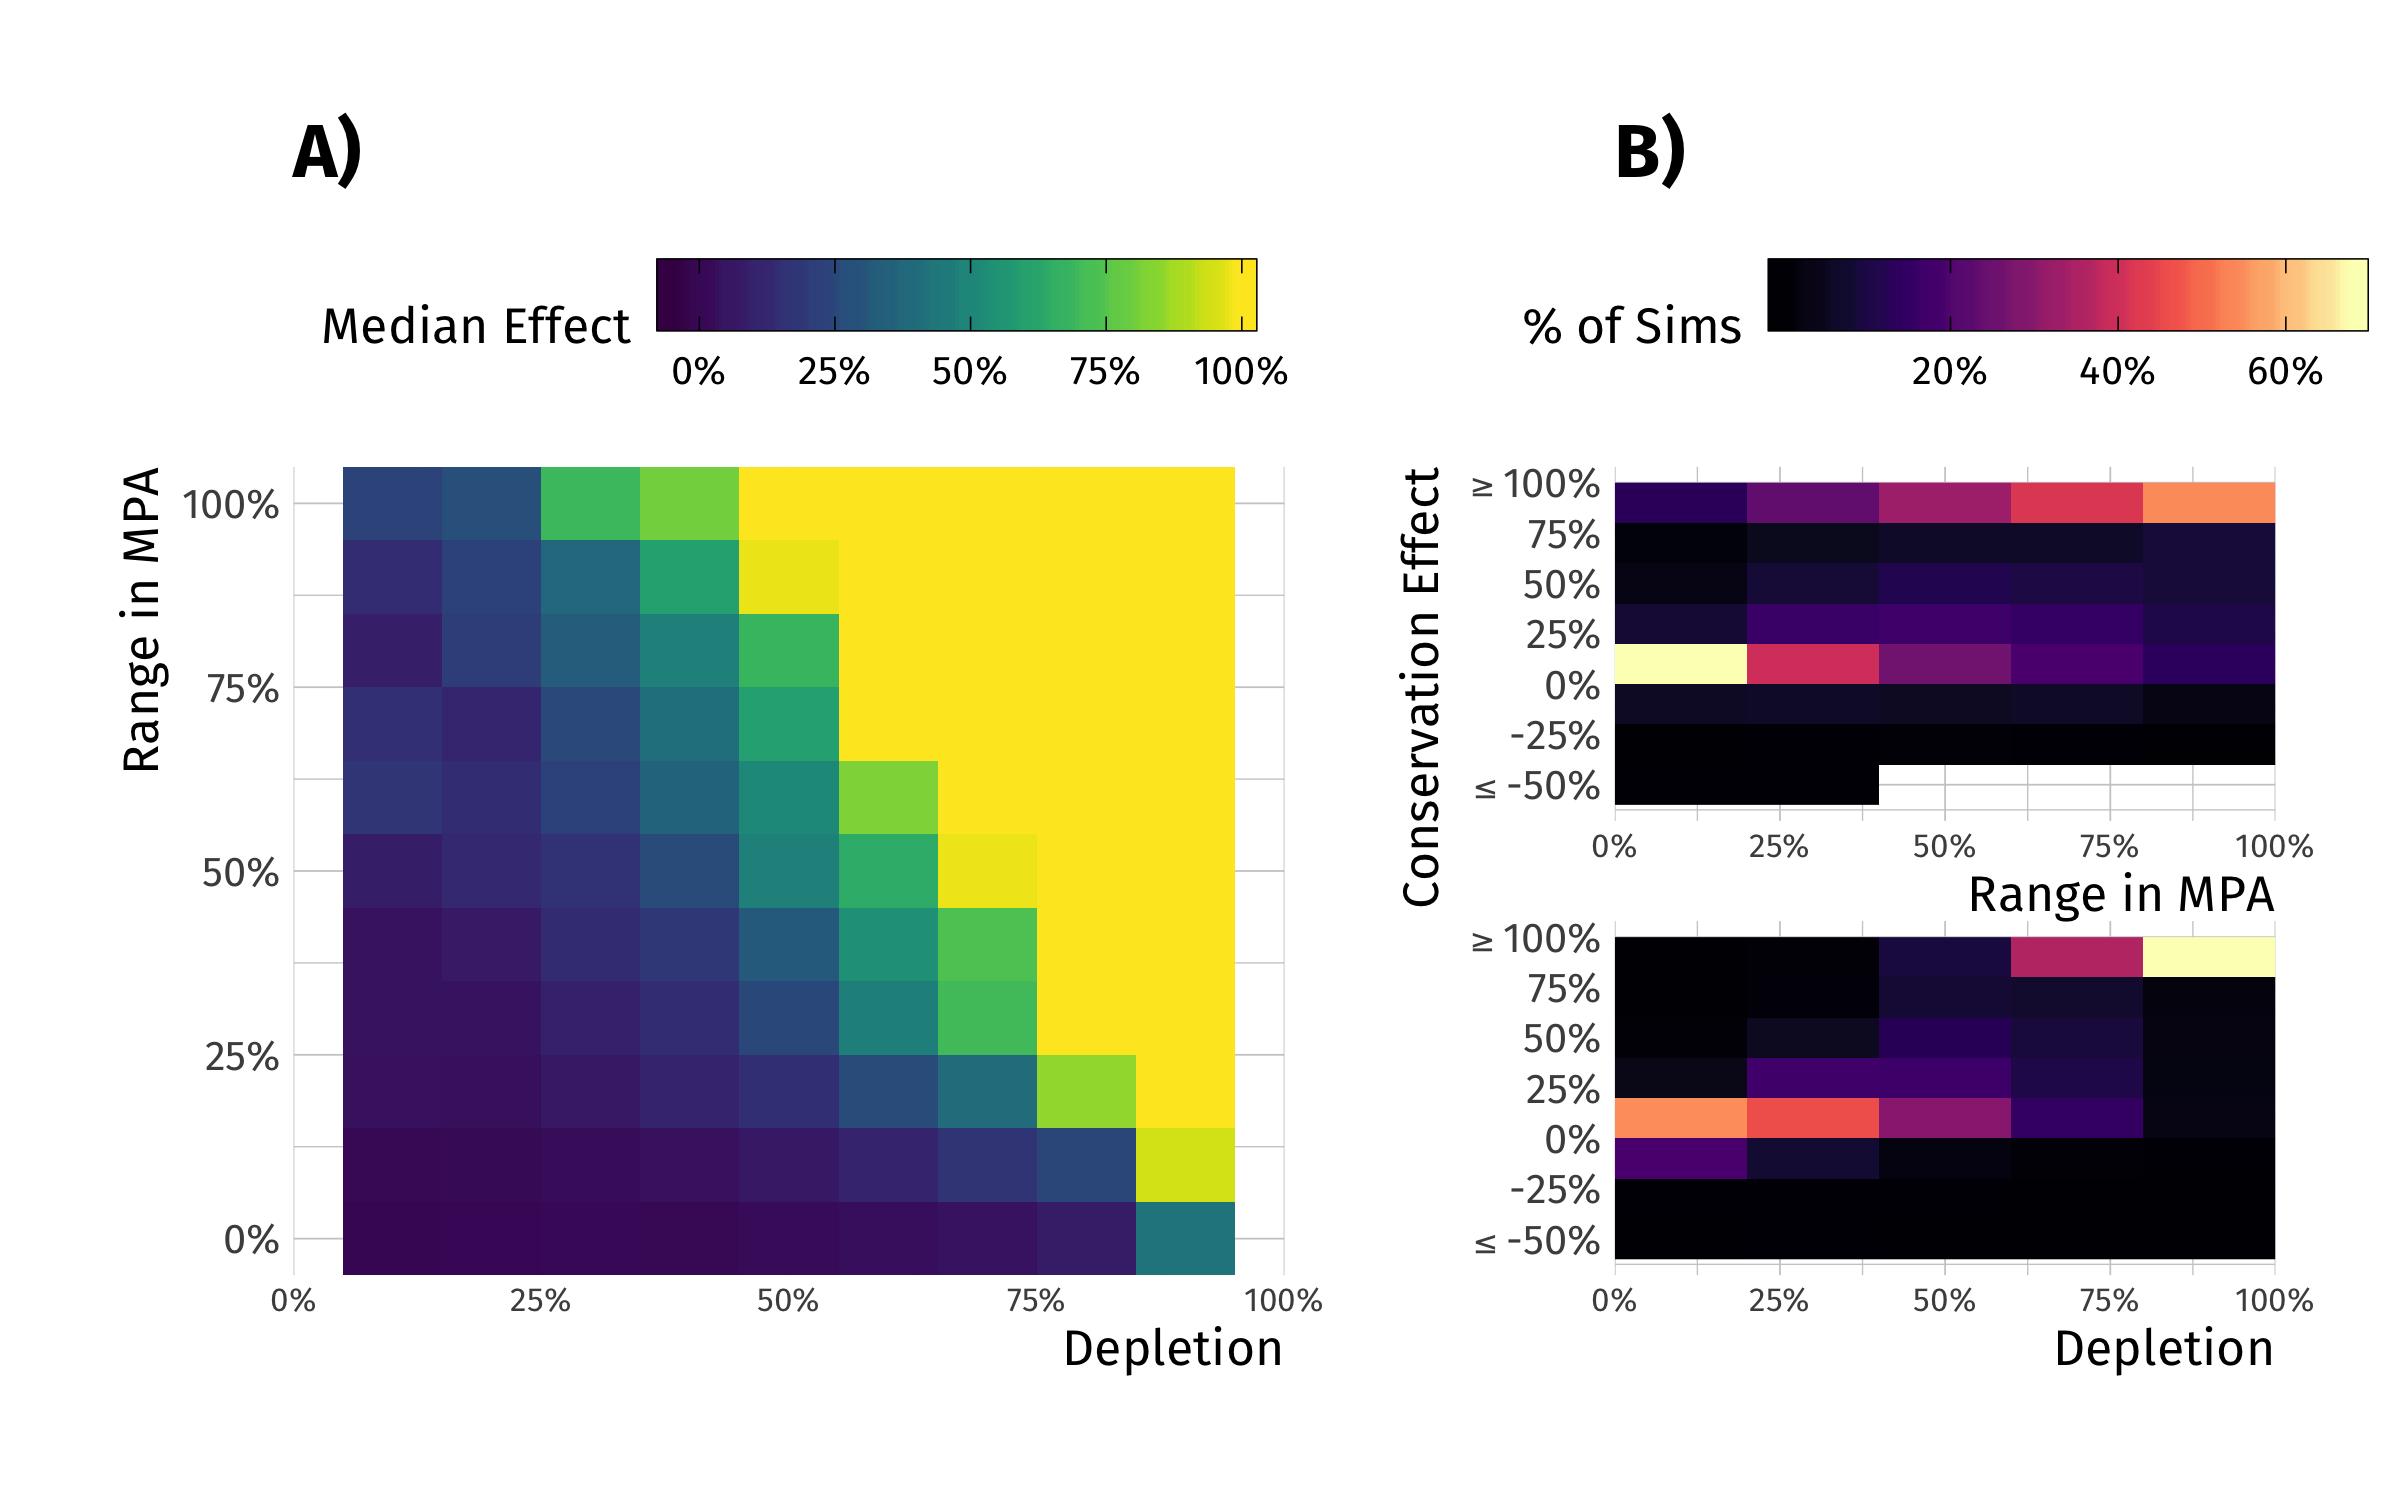
\includegraphics[width=.9\linewidth]{figs/conservation-effect.png}
  \caption{Median (A) and range (B) of equilibrium regional MPA conservation effects (percent change in total biomass with MPAs relative to without MPAs) across a range of depletion and MPA sizes (and incorporating the full range of scenarios included in our study). "Range in MPA" is the percent of patches covered by an MPA, "Depletion" is the depletion that would have occurred in equilibrium without the MPA. Colors in panel B represent the percentage of simulations that fell into an effect size bin at each x-axis bin, such that the sum of all percentages for a given x-axis bin is 1.}
  \label{conservation-effects}
\end{figure*}

\hypertarget{how-can-we-detect-regional-effects}{%
\subsection{How Can We Detect Regional
Effects?}\label{how-can-we-detect-regional-effects}}

How can we empirically measure the regional effects of MPAs? Intuition
and bio-economic theory tells us that the regional conservation effects
of MPAs are likely to be highly context dependent across locations and
across species within locations, so careful thought must be devoted to
an empirical design to detect their effects. The perfect experiment
would involve two parallel worlds that were identical, except for the
implementation of an MPA. In world ``A'', no MPA would be implemented,
and in the facsimile world ``B'', the MPA would be implemented. Both
worlds would be tracked before and after MPA implementation, and the
conservation and fishery outcomes would be compared after treatment.
Instead of two parallel worlds, a similar experimental design would
involve random placement of MPAs. Unfortunately, neither of these
experimental designs has been implemented, because parallel worlds do
not exist and MPAs are never placed at random. Careful causal inference
requires some other means of controlling for biases introduced by
factors such as the MPA siting process and biological spillover and
concentration of fishing effort (22, 41).

Conservation effects are typically estimated by comparing organism
densities or biomass inside MPAs to densities or biomass in selected
control sites outside MPAs, which we will refer to as response ratios.
(5) and (42) present meta-analyses of hundreds of such studies. These
results often find massively higher densities and biomasses inside MPAs
than outside (5). While response ratios are intended as a measure of the
effectiveness of reserves within their borders, these result stand in
contrast to the smaller region wide effect sizes predicted by our
simulation model. This raises the question: How reliable are density or
biomass ratios as estimators of regional conservation effects?

Control sites used in density or biomass ratios are often selected based
on abiotic or ecological traits such as habitat characteristics (22).
However, selection of control sites is further complicated by the very
spillover that MPAs are often intended to create. Export of adults or
larvae from the MPA to the ``control'' site affects their status as
controls, as does displacement of fishing effort from MPAs to control
sites. In theory, control sites far enough away to negate both
biological spillover and concentration by the fishing fleet could be
selected, but finding suitably far sites that are also appropriate
proxies for the ecological and economic context of the MPAs may be
challenging. While these concerns have been stated previously (43), the
MPA evaluation literature has by and large been unable to adequately
address them, often due to the very real challenges of acquiring the
necessary data (22).

Failure to account for these spillover effects can result in a biased
estimate of the true effect of a policy such as MPA placement (41). In
an ideal setting, the control site used in a response ratio would be a
perfect counterfactual for what would have occurred without the MPA. We
used our simulation model to approximate this scenario, calculating the
response ratio as the ratio of densities inside the MPAs relative to the
overall density from the paired simulation without MPAs multiplied by
the area of the population in an MPA (to account for the fact that we
would expect the effectiveness of a response ratio as a proxy for
regional conservation effects to scale with the size of the MPA relative
to the range of the species, Fig.\ref{density-ratio}-A). In this
idealized case, the response ratio is often a reasonable estimator for
the regional conservation effect.

What happens when the ``control'' sites are in fact affected by the
application of the MPA through biological spillover and fishing
concentration? In order to address this possibility, we calculated a new
response ratio as the mean density inside MPAs relative to the mean
density outside the MPAs (both weighted by distance from MPA borders and
scaled by MPA size). We only include simulations in which habitat and
larval dispersal rates are identical inside and outside of MPAs, to
approximate a scenario in which treatment and control sites have been
paired by ecological characteristics. Under these circumstances the
response ratio is a somewhat biased and very inaccurate estimator of the
true regional effect of MPAs. While on average high response ratios
correspond with high true regional effects, the variance is high, so the
response ratio alone cannot be used as a reliable proxy for the true
regional effect, without accounting for the sources of biases discussed
here. For higher movement rates, response ratios were frequently near
0\% (potentially leading stakeholders to conclude that the MPA had been
ineffective), when in fact in many cases the true effect of the MPA was
highly positive. For highly sedentary species, extremely high response
ratios could create the appearance of massive conservation gains when in
fact the net effect on the regional population has been near zero or
even negative (Fig.\ref{density-ratio}-B).

We note that spatial before-after-control-impact (BACI) studies present
a potential improvement over response ratios, controlling for
differences in mean densities in the treated and control regions as well
as MPA independent trends, but are much rarer due to the need for
extensive pre-MPA monitoring. However, spatial BACI still requires that
the MPAs do not affect the control sites, and as such has many of the
same limitations as response ratios as an estimator of regional
conservation effects.

To the extent that we can select control sites that are both
sufficiently similar to the region treated with MPAs and are unaffected
by biological or economic spillover, response ratios may be reliable
estimators of regional conservation effects. In reality these conditions
are unlikely to hold but for a few select cases. This become especially
difficult when networks of MPAs are implemented, such as has occurred in
California. In this case, control sites are generally located within a
few kilometers from MPA borders, making biological and economic
spillover highly likely. In these circumstances, without robust
statistical controls, response ratios may provide an unreliable estimate
of the regional conservation effect of marine protected areas.

\begin{figure*}%[tbhp]
  \centering
  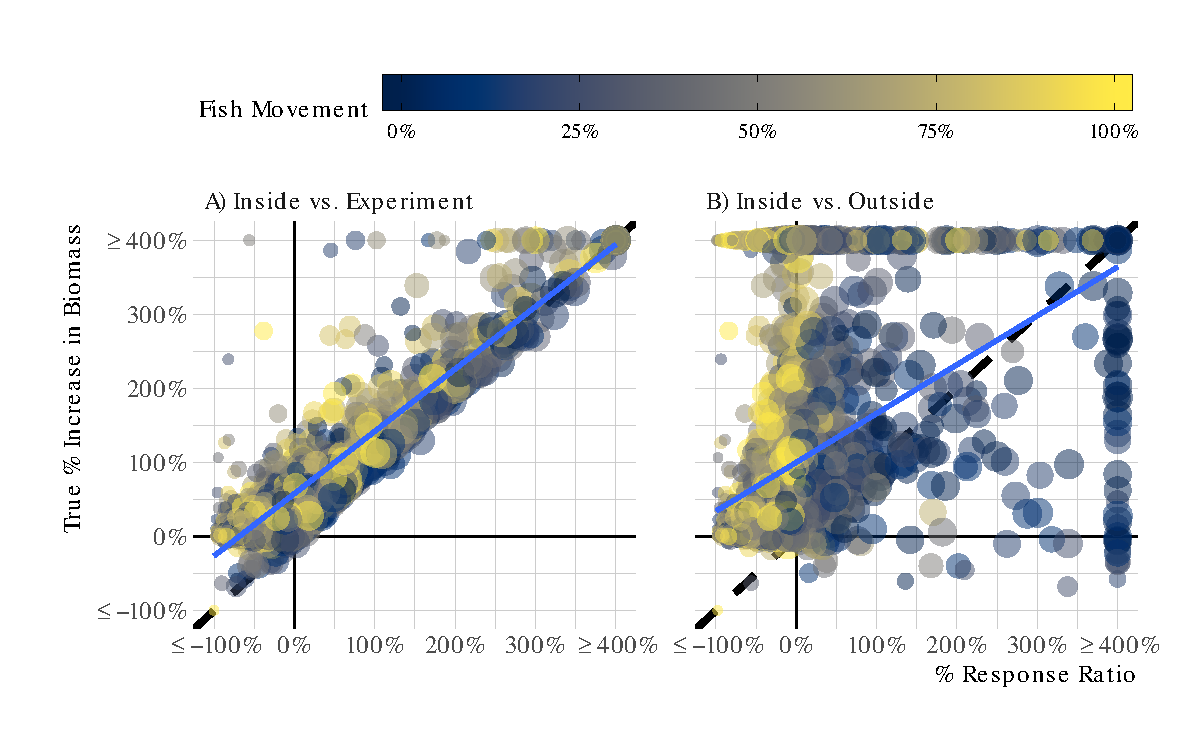
\includegraphics[width=.9\linewidth]{figs/density-ratio.pdf}
  \caption{Simulated MPA-size weighted response ratios (x-axis) plotted against true regional change in biomass caused by MPAs (y-axis). Each point represents a simulation, and color represents the movement rate of fish in the simulation (expressed as a percentage of the patches a fish is likely to move in one time step). The black line shows the one:one fit line, the blue line is a linear fit of the relationship between observed response ratios and true regional change in biomass. Inside vs. Experiment simulates a true control, while Inside Vs. Outside uses a control that may be affected by the treatment.}
  \label{density-ratio}
\end{figure*}

\hypertarget{estimating}{%
\subsection*{MPA Effects in the Channel Islands}\label{estimating}}
\addcontentsline{toc}{subsection}{MPA Effects in the Channel Islands}

\begin{figure}%[tbhp]
  \centering
  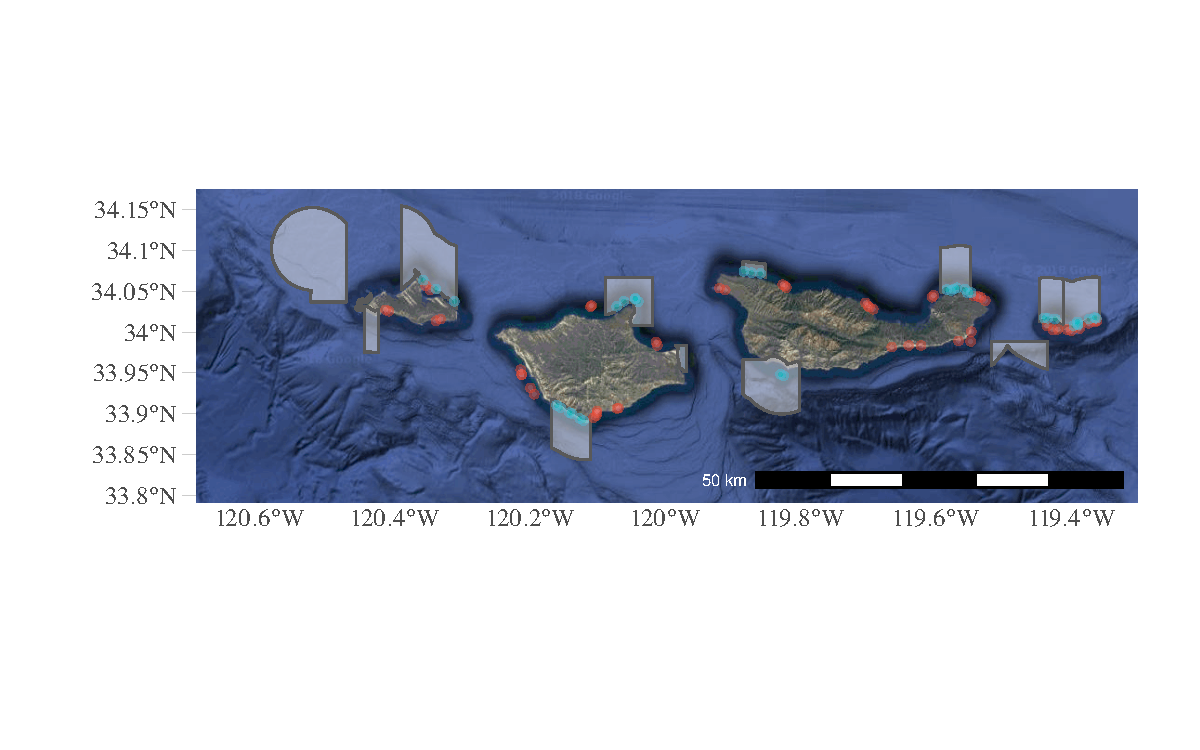
\includegraphics[width=1\linewidth]{figs/channel-islands.pdf}
  \caption{Map of PISCO sampling locations within the the Channel Islands National Marine Sanctuary, California, USA. Grey boxes indicated MPAs, points sampling locations, with color representing whether the site is inside an MPA (blue) or not (red)}
  \label{channel-islands}
\end{figure}

Given these challenges, what is a viable alternative for estimating the
conservation effects of MPAs? In a manner similar to (38), we use a
difference-in-difference estimator comparing densities in finfish
species targeted by fishing effort (i.e., those potentially affected by
an MPA) from those not targeted before and after MPA implementation
(41). Targeted species in the Northern Channel Islands, California,
include commercially important finfish such as California sheephead
(\emph{Semicossyphus pulcher}), and copper (\emph{Sebastes caurinus})
and blue (\emph{Sebastes mystinus}) rockfish. Each of these targeted
species was the subject of prior bio-economic modeling related to the
effects of MPAs in southern California (44, 45). But, we must note that
the analysis omits species from important invertebrate fisheries
including red urchin (\emph{Mesocentrotus franciscanus}) and spiny
lobster (\emph{Panulirus interruptus}). Non-targeted species include
garibaldi (\emph{Hypsypops rubicundus}), halfmoons (\emph{Medialuna
californiensis}), and blacksmith (\emph{Chromis punctipinnis}) (See
Table.S2 for a complete list of species). The key assumptions of this
approach are that a) within the time-frame of the model there are no
significant interaction effects between the targeted and non-targeted
species (which in fact we do not detect, see SI section 1.6.3), and b)
that in the absence of the MPAs both the targeted and non-targeted
groups of species would have exhibited similar trends in densities (the
parallel-trends assumption). The advantage to this approach is that
given the time-frame of the model (15 years), we believe that spillover
effects of MPA placement on the non-targeted species are likely to be
much less severe than the effects of biological spillover and fishing
concentration that may bias the performance of estimators such as a
response ratios or a spatial BACI design.

We applied this difference-in-difference strategy to a large dataset in
California. We used empirical kelp forest survey data from the
Partnership for Interdisciplinary Studies of Coastal Oceans (PISCO)
monitoring in the Northern Channel Islands with the ultimate goal of
testing the regional effects of MPAs in a real world context. A network
of MPAs covering approximately 20\% of the islands' waters was put in
place in 2003 as part of the California Marine Life Protection Act
(MLPA) (see (46), (47), (48), and (49) for information on the creation
of the MLPA). PISCO conducts visual SCUBA surveys at a large number of
rocky-reef and kelp forest sites inside and outside of MPAs throughout
the Channel Islands, producing estimates of densities of fishes that are
both targeted and non-targeted by fishing
(Fig.\ref{channel-islands}-\ref{pop-trends}).

Although the Islands do not encompass the full population of any of
these species, they encompass a large enough area to assess the regional
MPA conservation effects we might see in the Channel Islands after 13
years of protection (the time span covered by our model). The median
regional conservation effect produced by our simulation model after 13
years of protection by MPAs covering between 15\%-20\% of a population's
range was 25\%. This projected effect has an an interquartile range of
8\% and 100\%, although values as high as a 200\% increase and as low as
a 50\% decrease were also produced. Our expectation then is that all
else being equal we are likely looking for a modest but positive effect
size.

\begin{figure}%[tbhp]
  \centering
  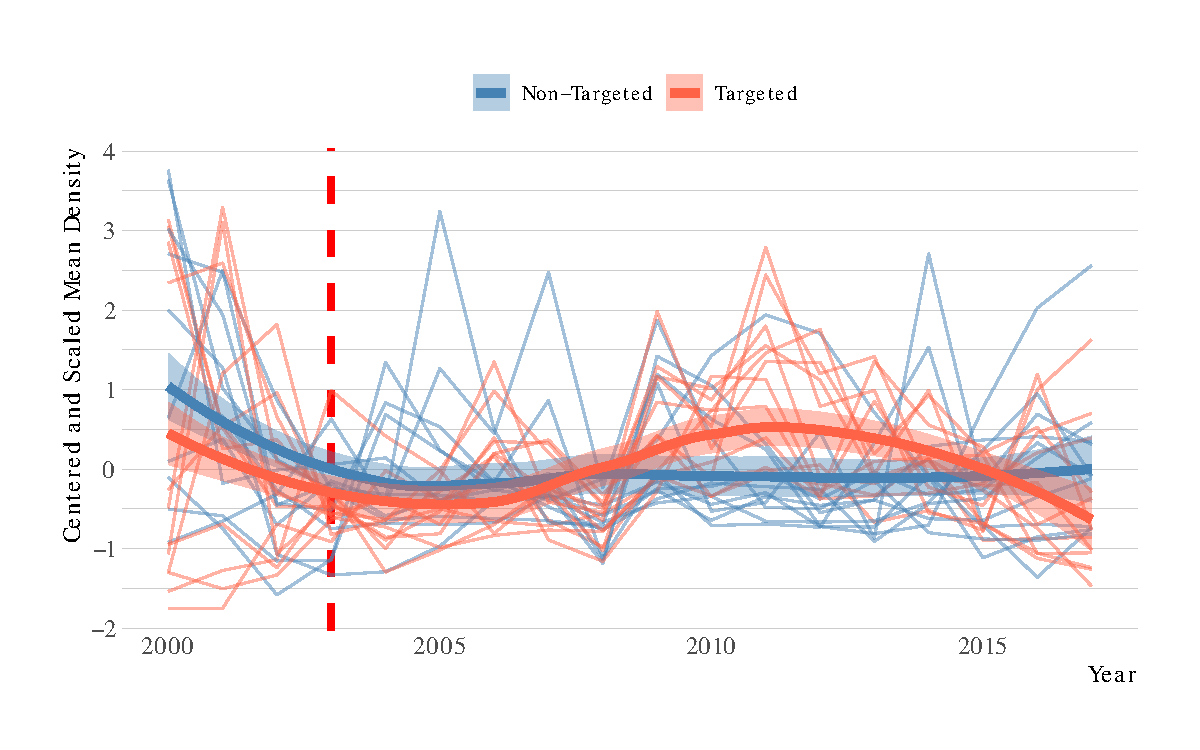
\includegraphics[width=1\linewidth]{figs/pop-trends.pdf}
  \caption{Centered and scaled mean annual biomass densities of included targeted (red) and non-targeted (blue) fish species (faded lines) and smoothed means with 95\% confidence intervals over time (darker lines and ribbons).}
  \label{pop-trends}
\end{figure}

The raw trends in the biomass densities appear to show parallel trends
in the densities of targeted and non-targeted fishes pre-MPA, with the
targeted group diverging first positively and then negatively over time
(Fig.\ref{pop-trends}). However, these raw trends could be caused by any
number of confounding variables besides the effects of the MPAs
themselves, from changes in observer skill and sampling locations, to
shifts in environmental conditions. Using our difference-in-difference
model in an effort to control for these factors, we found no significant
difference in the biomass densities of targeted and non-targeted fishes
pre-MPA (before 2003), which provides support for the parallel trends
assumption critical to the difference-in-difference method. Following
the implementation of the MPAs in 2003, we see evidence of an increasing
trend in densities of targeted relative to non-targeted fish, reaching a
peak value in 2014. Following 2014, densities of targeted species appear
to have declined relative to what we would expect based on the
non-targeted group (Fig.\ref{did-plot}).

\begin{figure}%[tbhp]
  \centering
  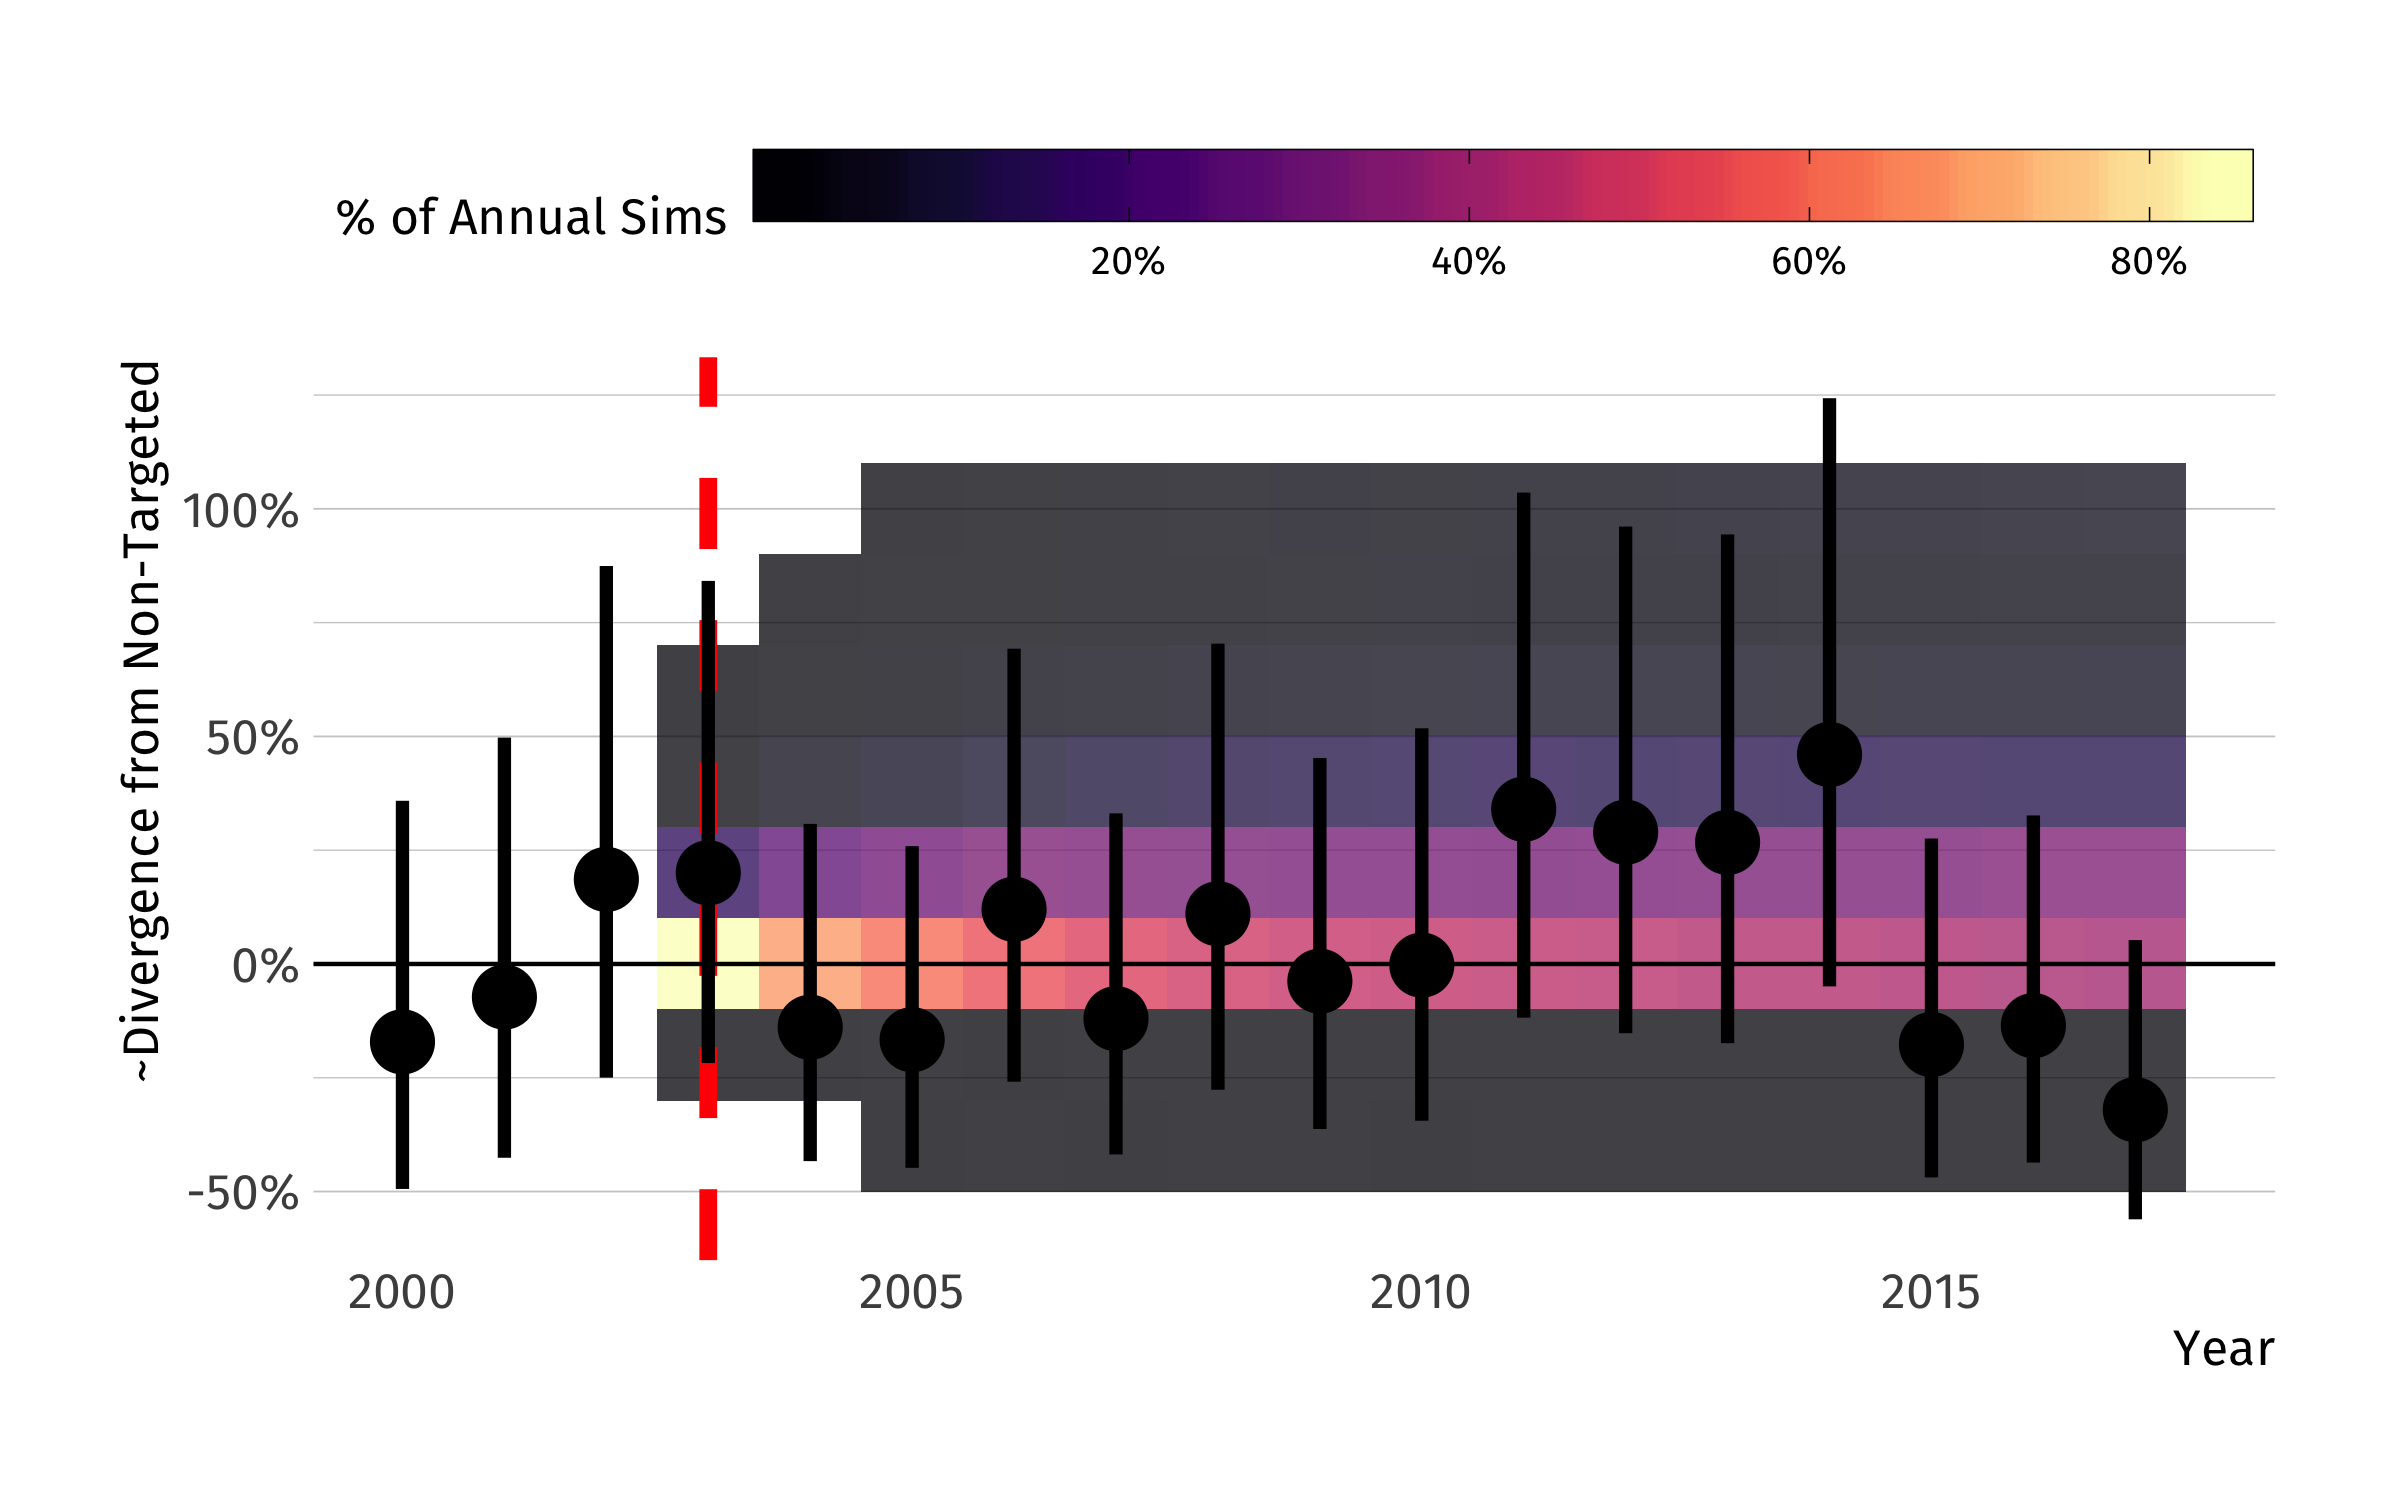
\includegraphics[width=1\linewidth]{figs/did_plot.png}
  \caption{Estimated divergence in biomass densities of targeted and non-targeted fishes throughout the Channel Islands (integrated across inside and outside of MPAs). MPAs are implemented in 2003 (red dashed line). Estimates are from a regression on log(biomass density), so estimated effects roughly correspond to percentage changes. Colored cells in the background indicate the frequency of MPA conservation effects predicted by our simulation modeling for MPAs similar in design and species composition to the Channel Islands.}
  \label{did-plot}
\end{figure}

\hypertarget{discussion}{%
\subsection*{Discussion}\label{discussion}}
\addcontentsline{toc}{subsection}{Discussion}

MPAs are an important part of the marine resource management toolbox.
Under ideal circumstances they can protect individual species and
ecosystem linkages, while supporting local economies through tourism and
fishing opportunities. One rationale for the expansion of MPAs is that
they will deliver net conservation benefits both inside \emph{and
outside} their borders. To date, this assumption is insufficiently
tested, and this is the focus of our paper. Our results show that
regional conservation benefits of MPAs are highly context dependent and
in many circumstances, are likely to be so small that they are nearly
impossible to detect empirically. Indeed, this is exactly what we found
in our empirical case study from the Channel Islands, California, USA.

We find regional conservation gains from MPAs in 94\% of our simulations
(Fig.\ref{conservation-effects}). MPAs covering less than 25\% of the
population range were unlikely to produce regional conservation gains
above 10\% unless the stock would have been severely overfished without
the MPA. Given that few marine species on the planet have more than 25\%
of their entire range protected in MPAs, this suggests that large
regional gains are unlikely to be common unless the overall extent of
MPAs grows globally. Large MPAs protecting highly depleted stocks almost
always produced large regional conservation gains, as should be
expected. The median conservation effect of 36\% stands in contrast to
the large within-MPA effects on biomass densities reported by (50) and
(5). This difference is due in part to the fact that within-MPA effects
are likely to be much larger than regional-MPA effects, but may also
reflect the many challenges of translating response ratios into regional
conservation effects. Our simulation analysis shows that without proper
controls (in particular for the effects of fleet redistribution),
response ratios well over 100\% are entirely plausible even when the
actual conservation effect is much lower (and \emph{vice versa}).

We were not able to detect a statistically significant difference in the
densities of targeted and non-targeted finfish species over the 13 years
of MPA protection in the Channel Islands covered by our analysis. The
data (and model assumptions) provide support for both negative and
positive MPA effects, although the size of these estimated effects is
well within the range that our simulation analysis suggests are
plausible. At face value, this lack of a clear result may seem
surprising given the size and carefully studied nature of this MPA
network.

However, our simulation analysis suggests that this result should
perhaps be expected. The Channel Islands MPAs cover approximately 20\%
of the waters in the Channel Islands, and while formal stock assessments
are not available for many of the targeted species in our analysis, what
evidence we have suggests that, as a group, these fish are on average
not heavily overfished. Some species, such as California sheephead and
blue rockfish were likely below target levels during the period (51,
52), but projections based upon the overall average response across all
species will likely suggest modest benefits even if a subset of species
could experience much larger population gains. Harkening back to our
simulations, we expect the average percentage difference in densities of
targeted species with and without MPAs to be modest
(Fig.\ref{did-plot}). Effects of this size are likely to be challenging
to detect empirically given the large natural variation of marine
ecosystems (especially temperate reefs) and the observation error
inherent in infrequent annual survey programs such as those provided by
PISCO.

In addition, our simulations examine percentage increases in biomass
densities. As an extreme example, an increase in biomass densities from
2kg/m\textsuperscript{2} to 4kg/m\textsuperscript{2} would be reported
as a 100\% increase. While this chance produces a large percentage
increase, this is a small change in absolute biomass densities relative
to the variance in the observation process itself (see Fig.S1 for a
companion to Fig.\ref{conservation-effects} scaled by absolute
population size). Beyond these challenges, the median estimated age at
sexual maturity for the targeted species included in this study is 5
years, meaning that the span of this analysis represents less than three
generations of MPA protection for half of the the measured species.
Ongoing monitoring may yet reveal clearer effects. Analysis of more
rapidly growing and maturing species, e.g.~spiny lobster, may also
reveal clearer signals.

While the MPA effect estimated by our model was not significant in any
one year, the positive trend from 2005 to 2014 is evident, as is the
sharp decline from 2015-2017. To what should we attribute this apparent
shift? We cannot reject the parallel trends assumption between the
targeted and non-targeted species in the years before the MPAs
(Fig.\ref{did-plot}). But, the Channel Islands region (and the entire
West coast of the USA) experienced a dramatic `marine heatwave'
beginning in 2014 and persisting through 2016, resulting in part in
extremely elevated water temperatures throughout the region (53).
Biogeographic differences in the distributions of targeted and
non-targeted species may confound the observed effects of MPAs. Many of
the non-targeted species have warm thermal affinities and have increased
in numbers since the heatwave (54). However, the targeted group is made
up mostly of fishes with cold-water affinities, such as members of the
genus Sebastes. As such, we hypothesize that the recent evidence for a
decline in densities of targeted species is due to environmental
conditions that disproportionately affect the targeted group (and not
for example due to concentrated fishing pressure outside the reserves).
This hypothesis is supported by the sharp declines in densities of
targeted species seen inside the MPAs themselves (see Fig.S27-S29),
suggesting a driver other than fishing may be at play. The Channel
Islands case study demonstrates the challenge of detecting small effect
sizes in nature and highlights the potential for small effect sizes to
be overwhelmed by additional environmental shocks to the system.

What do our results imply about the future of MPA science? Our
simulation model is by no means exhaustive (for example it ignores
features such as species interactions, habitat effects, and climate
feedback), but captures many of the core factors theorized to affect MPA
performance. Our results show that while attributes such as MPA size and
fishing pressure are important factors in determining the effects of
protection, local fleet dynamics and the movement rates of adult fish
can dramatically affect the outcomes of protected areas as well
(Fig.\ref{conservation-effects}). Far from being a simple tool with
clear outcomes, the effects of MPAs can be highly context dependent,
requiring - we would argue - a bio-economic model of at minimum the
complexity presented here to help communities design and set
expectations of MPAs at the tactical level. While users may not be able
to parameterize every aspect of a model such as that presented here,
working with stakeholders to visualize the implications of, for example,
different fleet responses to MPA implementation is a critical step in
MPA design. Readers can use our simulation model to explore the effects
of MPAs through an interactive web application available
\href{https://danovando.shinyapps.io/simmpa/}{here}.

Once simulation models have been used to help design an MPA, how can
users evaluate whether it is achieving their objectives? Response ratios
are commonly used as evidence for conservation outcomes of MPAs (5), but
as suggested in (22) and (41) and demonstrated here, without careful
attention to the design of control sites (accounting for example for the
displacement of effort by MPAs), response ratios may be highly
unreliable estimators of regional MPA effects. As (41) suggests, there
are many potential alternatives for estimating the effects of MPAs that
better account for the challenges of causal inference. We applied one
such approach here (a difference-in-difference estimator), and yet were
still unable to reach robust conclusions as to the effect of MPAs on the
density of targeted species in the Channel Islands, due to the likely
small size of the true effect relative to the strength and variability
of environmental drivers.

While this does not mean that all MPAs will face similar challenges in
estimating their effects, our results in the rigorously studied Channel
Islands system make clear that in many instances empirically detecting a
clear regional effect of MPAs may not be possible. How then should
stakeholders go about adaptively monitoring and managing MPAs?
Simulation modeling can help inform the range of effect sizes that may
be expected, and monitoring programs can perhaps be tuned to focus on
the species groups that have the highest chance of a detectable effect
size (39). Expanding data collection to include robust monitoring of
fleet dynamics may help statistical approaches to isolate the true
effect of MPAs on conservation outcomes by allowing for improved control
of the effects of fishing dynamics, and allow managers to take into
account potential negative interactions between MPAs and fleet dynamics
such as those that may occur under constant-catch dynamics. Whenever
possible monitoring programs should be implemented prior to MPA
implementation to provide a pre-treatment benchmark. Non-equilibrium
analyses (Fig.\ref{did-plot}) also help set expectations for effect
sizes over time. Beyond that, educating communities about the challenges
of estimating the effects of MPAs can help set expectations, so that a
lack of a clear effect is not necessarily viewed as a failure of the
program, but rather considered in the context of reasonable
expectations. While this paper has focused on the conservation outcomes
of MPAs, future work must also address the challenge of predicting and
estimating the fishery impacts of protected areas.

As the number and size of global MPA networks increase, it is critical
that we both set appropriate expectations for their outcomes, and plan
how we will monitor the performance of these protected areas over time.
While the history of MPA science has made important strides in helping
us understand the dynamics of protected areas, the future of MPA science
must directly tackle the challenge of evaluating the performance of
these MPAs, and adapting their design as needed to best achieve
objectives. Commonly employed metrics such as response ratios may be
applicable in some circumstances, but can have severe shortcomings as
metrics of regional conservation effects. Dependence on unreliable
estimators of MPA effects may lead to stakeholders incorrectly
attributing negative environmental shocks as MPA failures, or
interpreting data arising from scorched earth fishing outside MPAs as a
conservation success. Bio-economic modeling can help frame community
expectations, reducing the potential for a reduction in support if
unrealistic conservation or fishery gains are not realized. Statistical
approaches that explicitly address complications such as the spatial
spillover effects of MPAs (such as the difference-in-difference approach
used here) may give users an improved understanding of the performance
of their MPAs. Effective use of simulation and statistics to clearly
communicate what we should expect and what we can detect from MPAs is
critical in ensuring that MPAs play effective roles in fisheries
management and marine conservation.

\hypertarget{materials-and-methods}{%
\subsection{Materials and Methods}\label{materials-and-methods}}

We present here critical characteristics of our simulation model and
regression approach. Further details can be found in the Supplementary
Information. All analysis were conducted in R (55). Our main
difference-in-difference model was fit using Template Model Builder in R
(56). A completely reproducible version of our results can be accessed
and run at XX.

\hypertarget{simulation-model}{%
\subsubsection{Simulation Model}\label{simulation-model}}

Our bio-economic model simulates the effect of MPAs on a spatially
explicit age-structured representation of a single species. Readers can
explore the functionality of the model using an online tool available
\href{https://danovando.shinyapps.io/simmpa/}{here}. See Table.S1 for a
complete description of simulation states. The model consists of 25
patches with wrapped edges (picture the waters around a circular
island). For any one simulation we randomly pull a species and its
associated life history (growth, mortality, maturity) from the
\texttt{FishLife} (57) package in R. We pair these data with randomly
selected values between 0.6 and 0.95 for Beverton-Holt steepness (58),
as well as larval and adult dispersal rates (where at the lowest values
adults and larvae stay within the patch they were created, and at the
highest values they are capable of moving throughout the system in each
time step). We also randomly assign whether adults have density
dependent movement (meaning that adult biomass preferentially moves
towards patches with lower adult biomass as opposed to random
dispersal), as well as one of three potential types of density
dependence (59):

\begin{enumerate}
\def\labelenumi{\arabic{enumi}.}
\item
  Local density dependence: Density dependence occurs independently in
  each patch, and recruits then disperse to nearby patches
\item
  Global density dependence: Density dependence is a function of the sum
  of spawning biomass across all patches, and recruits are then
  distributed according to habitat quality
\item
  Post-dispersal density dependence: Larvae are distributed throughout
  the system, and then density dependence occurs based on the density of
  adult biomass at the destination patch
\end{enumerate}

We allow for three potential siting strategies for MPAs. In the first,
MPAs are randomly placed. In the second, we assume that MPAs are placed
in preferentially better habit (unfished recruitment is four times
greater inside MPA locations). In the third, we allow for scenarios in
which MPAs are placed in hotspots of larval dispersal. In this scenario,
patches in which MPAs will be placed have larval dispersal rates four
times greater than patches that do not become MPAs.

Each simulation is assigned a random set of fleet dynamics from one of
three categories: constant-catch, constant harvest rate, or open-access.
Under constant-catch, the fleet attempts to catch a randomly selected
multiplier of maximum sustainable yield (MSY) each year (note that
values of MSY greater than 1 will crash the population eventually, but
allows for overfishing dynamics to be observed when shorter time periods
are considered). Under a constant harvest rate the fleet captures a
randomly selected fraction between 0.01\% and 98\% of the population in
each time step. Under open access, fishing effort is allowed to expand
and contract in response to the profitability of the fishery, where

\begin{equation}
  E_{t} = E_{t-1}\times\theta{PPUE_{t-1}}
  \label{eqn:oa}
\end{equation}

and

\begin{equation}
  PPUE{t} = \frac{\sum_{i=1}^{I}pCatch_{i,t} - cE_{i,t}^\beta}{\sum_{i=1}^I E_{i,t}}
  \label{eqn:profits}
\end{equation}

To shift the equilibrium of the open access model, we fix price \emph{p}
at 1 and \(\beta\) at 2, and adjust the cost parameter to achieve the
selected fishing mortality rate at bionomic equilibrium. These
combinations of fleet models allow each simulation to achieve randomly
selected levels of fishing pressure through different processes.

Along with the fleet dynamics model, each simulation is assigned a
random fleet dispersal scenario: uniform dispersal (where the total
effort of the fleet is divided evenly among all open patches), catch
dispersal (where the total effort of the fleet is divided according to
the catchable biomass in each available patch), and profit dispersal
(where the total effort of the fleet is divided according to the profit
per unit effort in each available patch).

Lastly each simulation is assigned an MPA scenario, defined by the
number and size of MPAs, the placement of those MPAs, and the year that
the MPAs are put in place. Many MPA models assume equilibrium conditions
prior to the MPA, and then measure equilibrium outcomes. While these are
important scenarios to understand, they do not reflect the reality of
many MPAs, which are often placed in non-equilibrium conditions, and
evaluated over the early years of their existence. Each simulation
starts the population off at unfished equilibrium and then beings to
apply the fleet model. The MPAs are then placed during the randomly
selected start year, allowing some runs to explore how the early
dynamics of the MPA play out when the fishery and population they are
placed on is not already at equilibrium. Fishing effort in displaced by
MPAs can either concentrate outside or leave the fishery.

Each simulation is run to equilibrium with and without the selected MPA
strategy (holding all else constant). We then measure the difference in
biomass and fishery catches in each time step in the scenario with and
without the MPAs to calculate the conservation and fishery effects of
the MPAs over time. We filter out any scenario that results in a
collapse of the population (biomass less than 10\% of unfished biomass)
prior to the implementation of MPAs, and any scenario in which the
open-access dynamics devolve into chaos.

\hypertarget{difference-in-difference-regression}{%
\subsubsection{Difference in Difference
Regression}\label{difference-in-difference-regression}}

We use a difference-in-difference regression style regression to attempt
to estimate the causal effect of MPAs on regional targeted fish biomass.
Empirically, this amounts to estimating the pre-post MPA difference in
the biomass densities of targeted species net the same difference for
non-targeted species in the Channel Islands.

The simplified form of this model is

\begin{equation}
  log(d_{i}) = \beta_0 + \beta_1T_{i} +  \beta_2MPA_{i} + \beta_{3}T_iMPA_i + e_{i}
\label{eq:did}
\end{equation}

where \(d_i\) is the biomass density at observation \emph{i}, \emph{T}
indicates whether the observation \emph{i} is for a targeted (\(T = 1\))
or non-targeted (\(T = 0\)) species, and \emph{MPA} marks whether
observation \emph{i} is in a pre MPA (\(MPA = 0\)) or post MPA
(\(MPA = 1\)) state. Under the assumptions of this model, \(\beta_3\) is
the causal effect of the treatment (\emph{MPA}) on the treated (targeted
species).

We briefly assess two of the most critical assumptions of this model
here: that the treated and non-treated groups have parallel trends, and
that the effect of the treatment on the treated does not tangentially
affect the untreated (i.e.~that the implementation of MPAs does not
indirectly affect the non-targeted group somehow). While the parallel
trends assumption cannot be formally proven, we can examine its validity
using the data from the years before the MPAs were put in place in 2003
(since after that we no longer expect the trends in the observed data to
be parallel). We do not detect any significant differences in the trends
of the biomass densities of the targeted and non-targeted species in the
years before the MPAs, meaning that we do not have evidence to reject
the assumption that densities of targeted and non-targeted species were
following similar trajectories before the MPAs (though the model does
not estimate a precise zero effect either).

With regards to the second assumption, all of the species in this
empirical analysis exist within an ecosystem, and as such affect each
other through mechanisms such as predation, competition, and habitat
modification. Conceivably then, protection of carnivorous targeted
species inside MPAs could drive down the density of non-targeted prey
species, serving in that case to positively bias our estimate of the
effect of MPAs on the targeted species. While we know dynamics such as
this have to exist on some level, we find it unlikely that these effects
have had enough time to manifest in the 13 years of post-MPA data used
in our analysis (60, 61).

We used convergent cross mapping (CCM), in the manner of (62), to test
for the possibility of the trophic cascades biasing our results.
Generalizations of Takens' theorem indicate that if two variables (in
our case, species or physical variables) are part of the same dynamic
system, their individual dynamics should reflect their relative causal
influence. In other words, if one variable is causally forced by
another, that forcing should leave a signature on the first time series.
Convergent cross mapping (CCM) tests for causation by using the
attractor/manifold built from the time series of one variable to predict
another (hence the ``cross-mapping''). In simple terms, the causal
effect of A on B is determined by how well B cross-maps A. CCM then
allows us to test for causal relationships in the timeseries of
densities of targeted and non-targeted species. Our results found no
significant cross-mappings between targeted and non-targeted species,
indicating that while clearly there are interactions between these
groups on some level, the effects within the timespan of the data are
not pronounced enough to be of concern to our results (see SI for
additional information in CCM testing). However, the longer MPAs are in
place, the greater the possibility that substantial species interactions
that can affect use of non-targeted species as a control may arise.

While Equation.\ref{eq:did} presents the general form of our model, in
practice the estimation model is much more involved. At the rawest
level, the data are counts of finfish in 2cm length bins along a 30m x
2m transect at various sites and depths. These length bins are converted
to biomass, and then biomass densities, by converting length to weights
using available allometric data and dividing by the transect area. Our
goal is to estimate the effect of the MPAs on these biomass densities of
fish throughout the Channel Islands. We fit this model using a
hierarchical mixed-effect framework using Template Model Builder (56) in
R. The model consists of three levels, the first (starting from the
``bottom'') being transect-level densities of fish species observed by
PISCO, which are standardized into a standardized biomass abundance
index, accounting for both probability of detection and expected density
as a result of changes in both abundance and covariates such as
visibility and observer experience (63). For the second stage, we break
the abundance indices into targeted and non-targeted species (per the
classifications in the PISCO data), and estimate the mean trend of each
group (targeted and non-targeted) over time. In the third step, we
estimate the difference in the de-meaned trend between the targeted and
non-targeted fishes (controlling for factors such as water temperature,
kelp cover, and commercial fishery catches), that under the assumptions
of the model reflects the causal effect of the MPAs on the outcome of
interest (in this case regional biomass density of targeted fishes). All
three of these steps are integrated into the same estimation model, in
order to propagate uncertainty through the model correctly. Simpler
versions of the estimation model, as well as a synthetic control
identification strategy, were assessed as well and showed results
consistent with the model in our main results (see SI).

\showacknow

~ ~ ~

\hypertarget{refs}{}
\leavevmode\hypertarget{ref-johannes1978}{}%
1. Johannes RE (1978) Traditional Marine Conservation Methods in Oceania
and Their Demise. \emph{Annual Review of Ecology and Systematics}
9(1):349--364.

\leavevmode\hypertarget{ref-iucn1976}{}%
2. IUCN (1976) \emph{IUCN yearbook, 1975-76 : Annual report of the
International Union for Conservation of Nature and Natural Resources for
1975 and for January-May 1976}.

\leavevmode\hypertarget{ref-watson2014b}{}%
3. Watson JEM, Dudley N, Segan DB, Hockings M (2014) The performance and
potential of protected areas. \emph{Nature} 515(7525):67--73.

\leavevmode\hypertarget{ref-gaines2010}{}%
4. Gaines SD, White C, Carr MH, Palumbi SR (2010) Designing Marine
Reserve Networks for Both Conservation and Fisheries Management.
\emph{Proceedings of the National Academy of Sciences}
107(43):18286--18293.

\leavevmode\hypertarget{ref-lester2009}{}%
5. Lester S, et al. (2009) Biological effects within no-take marine
reserves: A global synthesis. \emph{Marine Ecology Progress Series}
384:33--46.

\leavevmode\hypertarget{ref-halpern2003}{}%
6. Halpern BS, Warner RR (2003) Review Paper. Matching marine reserve
design to reserve objectives. \emph{Proceedings of the Royal Society of
London Series B: Biological Sciences} 270(1527):1871--1878.

\leavevmode\hypertarget{ref-edgar2014}{}%
7. Edgar GJ, et al. (2014) Global conservation outcomes depend on marine
protected areas with five key features. \emph{Nature} 506(7487):216.

\leavevmode\hypertarget{ref-gerber2005}{}%
8. Gerber LR, Heppell SS, Ballantyne F, Sala E (2005) The role of
dispersal and demography in determining the efficacy of marine reserves.
\emph{Canadian Journal of Fisheries and Aquatic Sciences}
62(4):863--871.

\leavevmode\hypertarget{ref-goni2010}{}%
9. Goni R, Hilborn R, D\textbackslash{}'ıaz D, Mallol S, Adlerstein S
(2010) Net contribution of spillover from a marine reserve to fishery
catches. \emph{Mar Ecol Prog Ser} 400:233--243.

\leavevmode\hypertarget{ref-halpern2009}{}%
10. Halpern BS, Lester SE, Kellner JB (2009) Spillover from marine
reserves and the replenishment of fished stocks. \emph{Environmental
Conservation} 36(04):268--276.

\leavevmode\hypertarget{ref-kay2012}{}%
11. Kay MC, Lenihan HS, Kotchen MJ, Miller CJ (2012) Effects of marine
reserves on California spiny lobster are robust and modified by
fine-scale habitat features and distance from reserve borders.
\emph{Marine Ecology Progress Series} 451:137--150.

\leavevmode\hypertarget{ref-stobart2009}{}%
12. Stobart B, et al. (2009) Long-term and spillover effects of a marine
protected area on an exploited fish community. \emph{Marine Ecology
Progress Series} 384:47--60.

\leavevmode\hypertarget{ref-mcclanahan2000}{}%
13. McClanahan TR, Mangi S (2000) Spillover Of Exploitable Fishes From A
Marine Park And Its Effect On The Adjacent Fishery. \emph{Ecological
Applications} 10(6):1792--1805.

\leavevmode\hypertarget{ref-russ1996}{}%
14. Russ G, Alcala A (1996) Do marine reserves export adult fish
biomass? Evidence from Apo Island, central Philippines. \emph{Marine
Ecology Progress Series} 132:1--9.

\leavevmode\hypertarget{ref-thompson2017}{}%
15. Thompson AR, Chen DC, Guo LW, Hyde JR, Watson W (2017) Larval
abundances of rockfishes that were historically targeted by fishing
increased over 16 years in association with a large marine protected
area. \emph{Royal Society Open Science} 4(9):170639.

\leavevmode\hypertarget{ref-baetscher2019}{}%
16. Baetscher DS, et al. (2019) Dispersal of a nearshore marine fish
connects marine reserves and adjacent fished areas along an open coast.
\emph{Molecular Ecology} 28(7):1611--1623.

\leavevmode\hypertarget{ref-pelc2009}{}%
17. Pelc R, Baskett M, Tanci T, Gaines S, Warner R (2009) Quantifying
larval export from South African marine reserves. \emph{Marine Ecology
Progress Series} 394:65--78.

\leavevmode\hypertarget{ref-costa2013}{}%
18. Costa BH e, et al. (2013) Fishers' Behaviour in Response to the
Implementation of a Marine Protected Area. \emph{PLOS ONE} 8(6):e65057.

\leavevmode\hypertarget{ref-mason2012}{}%
19. Mason J, Kosaka R, Mamula A, Speir C (2012) Effort changes around a
marine reserve: The case of the California Rockfish Conservation Area.
\emph{Marine Policy} 36(5):1054--1063.

\leavevmode\hypertarget{ref-murawski2005}{}%
20. Murawski SA, Wigley SE, Fogarty MJ, Rago PJ, Mountain DG (2005)
Effort distribution and catch patterns adjacent to temperate MPAs.
\emph{ICES Journal of Marine Science} 62(6):1150--1167.

\leavevmode\hypertarget{ref-mcdermott2019}{}%
21. McDermott GR, Meng KC, McDonald GG, Costello CJ (2019) The blue
paradox: Preemptive overfishing in marine reserves. \emph{Proceedings of
the National Academy of Sciences} 116(12):5319--5325.

\leavevmode\hypertarget{ref-ferraro2018}{}%
22. Ferraro PJ, Sanchirico JN, Smith MD (2018) Causal inference in
coupled human and natural systems. \emph{Proceedings of the National
Academy of Sciences}:201805563.

\leavevmode\hypertarget{ref-gaines2003}{}%
23. Gaines SD, Gaylord B, Largier JL (2003) Avoiding Current Oversights
in Marine Reserve Design. \emph{Ecological Applications} 13(sp1):32--46.

\leavevmode\hypertarget{ref-botsford2008}{}%
24. Botsford LW, et al. (2008) Connectivity, sustainability, and yield:
Bridging the gap between conventional fisheries management and marine
protected areas. \emph{Reviews in Fish Biology and Fisheries}
19(1):69--95.

\leavevmode\hypertarget{ref-difranco2018}{}%
25. Di Franco A, et al. (2018) Linking home ranges to protected area
size: The case study of the Mediterranean Sea. \emph{Biological
Conservation} 221:175--181.

\leavevmode\hypertarget{ref-hilborn2004}{}%
26. Hilborn R, Punt AE, Orensanz J (2004) Beyond band-aids in fisheries
management: Fixing world fisheries. \emph{Bulletin of Marine Science}
74(3):493--507.

\leavevmode\hypertarget{ref-hilborn1992}{}%
27. Hilborn R (1992) Can fisheries agencies learn from experience?
\emph{Fisheries} 17(4):6--14.

\leavevmode\hypertarget{ref-walters2004}{}%
28. Walters CJ, Martell SJ (2004) \emph{Fisheries ecology and
management} (Princeton University Press).

\leavevmode\hypertarget{ref-hastings2003}{}%
29. Hastings A, Botsford LW (2003) Comparing Designs Of Marine Reserves
For Fisheries And For Biodiversity. \emph{Ecological Applications}
13(sp1):65--70.

\leavevmode\hypertarget{ref-gerber2003}{}%
30. Gerber LR, et al. (2003) Population Models For Marine Reserve
Design: A Retrospective And Prospective Synthesis. \emph{Ecological
Applications} 13(sp1):47--64.

\leavevmode\hypertarget{ref-hilborn2004a}{}%
31. Hilborn R, et al. (2004) When can marine reserves improve fisheries
management? \emph{Ocean \& Coastal Management} 47(34):197--205.

\leavevmode\hypertarget{ref-botsford2003}{}%
32. Botsford LW, Micheli F, Hastings A (2003) Principles for the Design
of Marine Reserves. \emph{Ecological Applications} 13(sp1):25--31.

\leavevmode\hypertarget{ref-costello2010}{}%
33. Costello C, Lynham J, Lester SE, Gaines SD (2010) Economic
incentives and global fisheries sustainability. \emph{Resource} 2.

\leavevmode\hypertarget{ref-fao2018}{}%
34. FAO (2018) \emph{The State of World Fisheries and Aquaculture 2018:
Meeting the sustainable development goals} (FAO, Rome, Italy).

\leavevmode\hypertarget{ref-costello2012}{}%
35. Costello C, Gaines S, Gerber LR (2012) Conservation science: A
market approach to saving the whales. \emph{Nature} 481(7380):139--140.

\leavevmode\hypertarget{ref-rosenberg2017}{}%
36. Rosenberg AA, et al. (2017) Applying a New Ensemble Approach to
Estimating Stock Status of Marine Fisheries around the World.
\emph{Conservation Letters}:n/a--n/a.

\leavevmode\hypertarget{ref-starr2015}{}%
37. Starr RM, et al. (2015) Variation in Responses of Fishes across
Multiple Reserves within a Network of Marine Protected Areas in
Temperate Waters. \emph{PLoS ONE} 10(3):e0118502.

\leavevmode\hypertarget{ref-caselle2015}{}%
38. Caselle JE, Rassweiler A, Hamilton SL, Warner RR (2015) Recovery
trajectories of kelp forest animals are rapid yet spatially variable
across a network of temperate marine protected areas. \emph{Scientific
reports} 5:14102.

\leavevmode\hypertarget{ref-nickols2019}{}%
39. Nickols KJ, et al. (2019) Setting ecological expectations for
adaptive management of marine protected areas. \emph{Journal of Applied
Ecology} 0(0).
doi:\href{https://doi.org/10.1111/1365-2664.13463}{10.1111/1365-2664.13463}.

\leavevmode\hypertarget{ref-villasenor-derbez2019}{}%
40. Villaseñor-Derbez JC, et al. (2019) An interdisciplinary evaluation
of community-based TURF-reserves. \emph{PLOS ONE} 14(8):e0221660.

\leavevmode\hypertarget{ref-larsen2019}{}%
41. Larsen AE, Meng K, Kendall BE (2019) Causal analysis in
controlImpact ecological studies with observational data. \emph{Methods
in Ecology and Evolution} 0(0).
doi:\href{https://doi.org/10.1111/2041-210X.13190}{10.1111/2041-210X.13190}.

\leavevmode\hypertarget{ref-halpern2002}{}%
42. Halpern BS, Warner RR (2002) Marine reserves have rapid and lasting
effects. \emph{Ecology Letters} 5(3):361--366.

\leavevmode\hypertarget{ref-halpern2004}{}%
43. Halpern BS, Gaines SD, Warner RR (2004) Confounding effects of the
export of production and the displacement of fishing effort from marine
reserves. \emph{Ecological Applications} 14(4):1248--1256.

\leavevmode\hypertarget{ref-costello2010d}{}%
44. Costello C, et al. (2010) The value of spatial information in MPA
network design. \emph{Proceedings of the National Academy of Sciences}
107(43):18294--18299.

\leavevmode\hypertarget{ref-rassweiler2014}{}%
45. Rassweiler A, Costello C, Hilborn R, Siegel DA (2014) Integrating
scientific guidance into marine spatial planning. \emph{Proceedings of
the Royal Society B: Biological Sciences} 281(1781):20132252.

\leavevmode\hypertarget{ref-osmond2010}{}%
46. Osmond M, Airame S, Caldwell M, Day J (2010) ``Lessons for marine
conservation planning: A comparison of three marine protected area
planning processes''. \emph{Ocean \& Coastal Management} 53(2):41--51.

\leavevmode\hypertarget{ref-kirlin2013}{}%
47. Kirlin J, et al. (2013) California's Marine Life Protection Act
Initiative: Supporting implementation of legislation establishing a
statewide network of marine protected areas. \emph{Ocean \& Coastal
Management} 74:3--13.

\leavevmode\hypertarget{ref-botsford2014}{}%
48. Botsford LW, White JW, Carr MH, Caselle JE (2014) Chapter Six -
Marine Protected Area Networks in California, USA. \emph{Advances in
Marine Biology}, Marine Managed Areas and Fisheries., eds Johnson ML,
Sandell J (Academic Press), pp 205--251.

\leavevmode\hypertarget{ref-hilborn2012}{}%
49. Hilborn R (2012) The role of science in MPA establishment in
California: A personal perspective. \emph{Environmental Conservation}
39(03):195--198.

\leavevmode\hypertarget{ref-halpern2003a}{}%
50. Halpern BS (2003) The impact of marine reserves: Do reserves work
and does reserve size matter? \emph{Ecological Applications}
13(sp1):117--137.

\leavevmode\hypertarget{ref-alonzo2004}{}%
51. Alonzo S, Key M, Ish T, MacCall AD (2004) \emph{Status of the
California Sheephead Stock for 2004}.

\leavevmode\hypertarget{ref-dick2017}{}%
52. Dick EJ, et al. (2017) \emph{The Combined Status of Blue and Deacon
Rockfishes in U.S. Waters off California and Oregon in 2017} (Pacific
Fishery Management Council, Portland, OR).

\leavevmode\hypertarget{ref-gentemann2017}{}%
53. Gentemann CL, Fewings MR, García-Reyes M (2017) Satellite sea
surface temperatures along the West Coast of the United States during
the 20142016 northeast Pacific marine heat wave. \emph{Geophysical
Research Letters} 44(1):312--319.

\leavevmode\hypertarget{ref-freedman2019}{}%
54. Freedman R (2019) Understanding the Efficacy of Spatial Management
on Emerging Threats. PhD thesis (University of California, Santa
Barbara).

\leavevmode\hypertarget{ref-rcoreteam2019}{}%
55. R Core Team (2019) R: A Language and Environment for Statistical
Computing.

\leavevmode\hypertarget{ref-kristensen2016}{}%
56. Kristensen K, Nielsen A, Berg CW, Skaug H, Bell BM (2016)
\textbf{TMB} : Automatic Differentiation and Laplace Approximation.
\emph{Journal of Statistical Software} 70(5).
doi:\href{https://doi.org/10.18637/jss.v070.i05}{10.18637/jss.v070.i05}.

\leavevmode\hypertarget{ref-thorson2017c}{}%
57. Thorson JT, Munch SB, Cope JM, Gao J (2017) Predicting life history
parameters for all fishes worldwide. \emph{Ecological
Applications}:n/a--n/a.

\leavevmode\hypertarget{ref-mace1994}{}%
58. Mace PM (1994) Relationships between Common Biological Reference
Points Used as Thresholds and Targets of Fisheries Management
Strategies. \emph{Canadian Journal of Fisheries and Aquatic Sciences}
51(1):110--122.

\leavevmode\hypertarget{ref-babcock2011}{}%
59. Babcock EA, MacCall AD (2011) How useful is the ratio of fish
density outside versus inside no-take marine reserves as a metric for
fishery management control rules? \emph{Canadian journal of fisheries
and aquatic sciences} 68(2):343--359.

\leavevmode\hypertarget{ref-babcock2010}{}%
60. Babcock RC, et al. (2010) Decadal trends in marine reserves reveal
differential rates of change in direct and indirect effects.
\emph{Proceedings of the National Academy of Sciences}
107(43):18256--18261.

\leavevmode\hypertarget{ref-pershing2015a}{}%
61. Pershing AJ, et al. (2015) Slow adaptation in the face of rapid
warming leads to collapse of the Gulf of Maine cod fishery.
\emph{Science} 350(6262):809--812.

\leavevmode\hypertarget{ref-clark2015}{}%
62. Clark AT, et al. (2015) Spatial convergent cross mapping to detect
causal relationships from short time series. \emph{Ecology}
96(5):1174--1181.

\leavevmode\hypertarget{ref-maunder2004}{}%
63. Maunder MN, Langley AD (2004) Integrating the standardization of
catch-per-unit-of-effort into stock assessment models: Testing a
population dynamics model and using multiple data types. \emph{Fisheries
Research} 70(23):389--395.



% Bibliography
% \bibliography{pnas-sample}

\end{document}

